%
%
\documentclass[10pt,a4paper,oneside]{book}

\usepackage[slovene]{babel}
\usepackage[utf8x]{inputenc}
\usepackage[fleqn]{amsmath}
\usepackage{amsfonts}
\usepackage{amssymb}
\usepackage{makeidx}
\usepackage{graphicx}

\usepackage{../torstyle}
%torstlye predloge:
%Definicija \Def{}
%Primer \Prim{}
%Prirejen itemize \begin{items}

\begin{document}
\begin{titlepage}
\begin{center}
\ \\[8cm]
{\huge Teoretične osnove računalništva}\\[1.5pt]
{\large Zapiski predavanj 2010/2011}\\[15pt]
{\large \today}
\vfill

\parbox{7.5cm}{
\begin{center}

\includegraphics[width=0.15\textwidth]{../CC}\\[5pt]

This work is licensed under a Creative Commons Attribution-NonCommercial-ShareAlike 3.0 Unported License
\end{center}
}
\end{center}
\end{titlepage}
\tableofcontents

%\newpage
%\section{Notacija}
%\begin{itemize}
%	\item[Množice:] Označimo z velikimi tiskanimi črkami. Podamo jih lahko na naslednje načine\\
%	$ A = \lbrace a_1, a_1, a_3, \ldots \rbrace $ - naštevanje elementov\\
%	$ B = \lbrace n | \ \mbox{pravilo za n} \rbrace \ $ - opis elementov
%\end{itemize}

\pagebreak
\chapter{Uvod}
\section{Dokazovaje}
\subsection{Dokaz s konstrukcijo}
Dokaz obstoja nekega objekta je to, da nam objekt uspe skonstruirati.

\begin{primeri}
\item Ali za vsako število elementov, večje od 4, obstaja graf ki ima natanko 3 liste?
%?manjka dokaz in slika
\item $| \mathbb{R} | = | [0,1) |$
%?manjka dokaz in še par podobnih je
\end{primeri}
	
\subsection{Dokaz z indukcijo}
Če je množica induktivni razred\footnote{Glej slovarček na koncu.}, lahko z matematično indukcijo dokazujemo neko lastnost članov množice.
\br
Induktivni razred $I$ sestavlja:
\begin{items}
\item Baza indukcije - najbolj osnovna množica elementov (osnovni razred)
\item Pravila generiranja - kako iz elementov baze gradimo nove elemente (množico)
\end{items}
\begin{primeri}
\item Induktivni razred naravnih števil $(\mathbb{N})$
	\begin{items}
	\item Baza: $1 \in \mathbb{N}$ 
	\item Pravila generiranja: $n \in \mathbb{N} \Longrightarrow n+1 \in \mathbb{N} $
	\end{items}
\item \fnurl{Hilbertove krivulje}{http://en.wikipedia.org/wiki/Hilbert_curve}
\end{primeri}

\subsection{Dokaz s protislovjem}
Vzamemo nasprotno trditev, od tiste, ki jo želimo preveriti in pokažemo, da to vodi v protislovje.

\begin{primeri}
\item Praštevil je končno mnogo
	\begin{items}
	\item Predpostavimo, da poznamo vsa praštevila:\\
		$P = \{2,3,5,...,p\}$, kjer je $p$ zadnje praštevilo 
	\item Po definiciji obstajajo le praštevila in sestavljena števila (to so taka, ki jih lahko razstavimo na prafaktorje). 
	\item Če pomnožimo vsa znana praštevila iz $P$ in prištejemo $1$ dobimo število, ki se ga ne da razstaviti na prafaktorje iz množice $P$:\\
		$q = 2 * 3 * 5 * ... * p + 1$
	\item Torej je $q$ ali praštevilo (ker ni sestavljeno), ali pa število, sestavljeno iz prafaktorjev, ki jih ni v množici $P$.
	\item Oboje kaže na to, da v množici $P$ nimamo vseh praštevil in da to velja za vsako končno množico praštevil.
	\end{items}
\item $\sqrt[3]{2}$ je racionalno število 
	\begin{items}
	\item $\sqrt[3]{2} = \frac{a}{b}$ ker je $\frac{a}{b}$ racionalen ulomek ga lahko okrajšamo in si ga od sedaj predstavljamo okrajšanega $GCD(a,b)=1$
	\item $ 2 = \left( \frac{a}{b} \right)^3 $
	\item $2b^3 = a^3$ tukaj vidimo da je a sodo število, torej lahko pišemo $ a = 2k $
	\item $2b = \left( 2k\right)^3 $
	\item $2b = 8k $
	\item $b = 4k $ ker je b tudi sodo število, vidimo da $GCD(a,b)=1$ ne drži, torej smo prišli v protislovje.
	\end{items}
\end{primeri}

\pagebreak
\chapter{Regularni jeziki}

\section{Uvod}
\subsection*{Oznake}
\begin{items}
\item $a$ - simbol oz. beseda dolžine 1
\item $\Sigma$ - abeceda oz. končna neprazna množica simbolov
\item $w$ - besede, nizi oz. poljubno končno zaporedje  simbolov $w_1w_2 \ldots w_n$. 
\item $|w|$ - dolžina niza - je $0$ za $w = \varepsilon$
\item $\varepsilon$ - prazen niz oz. niz dolžine $0$
\item $\Sigma^*$ - vse možne besede abecede
\end{items}

\subsection*{Operacije}
\begin{items}
\item Stik
	\begin{items}
	\item Stik nizov:
		\begin{align*}
		w  &= w_1 w_2 \ldots w_n\\
		x  &= x_1 x_2 \ldots x_m\\
		wx &= w_1 w_2 \ldots w_n x_1 x_2 \ldots x_m
		\end{align*}
	\item Stik množic:
		\begin{align*} 
		A & = \lbrace w_1 ,\ w_2 ,\ \ldots ,\ w_n \rbrace \\ 
		B & = \lbrace x_1 ,\ x_2 ,\ \ldots ,\ x_m \rbrace \\ 
		A \circ B & = \lbrace w_ix_j \ | \ w_i \in A \ \wedge \ x_i \in B \rbrace
		\end{align*} 
	\end{items}
\item Potenciranje
	\begin{align*} 
	A^0 & = \lbrace \varepsilon \rbrace \\
	A^k & = A \circ A \circ \cdots \circ A \ = \ \bigcirc_{i=0}^{k} A^i \\
	\end{align*}
\item Iteracija
	\begin{align*} 
	A^* &= A^0 \bigcup A^1 \bigcup A^2 \cdots  \ = \ \bigcup_{i=0}^{ \infty } A^i
	\end{align*} 		
\end{items}
\subsection*{Regularni jezik}
\Def{Regularni jezik $L$ nad abecedo $\Sigma$ je poljubna podmnožica $\Sigma^*$
	\begin{equation*} 
	L \subseteq \Sigma^*
	\end{equation*}
}
\begin{primeri} 
\item Prazen jezik: $L_1 =\lbrace \rbrace$
\item Jezik, ki vsebuje $\varepsilon$ (ni prazen): $L_2 = \lbrace \varepsilon \rbrace$
\item Jezik, ki vsebuje nize "a, aa, ab": $L_3 = \lbrace a, aa, ab \rbrace$
\end{primeri} 
\section{Regularni Izrazi}
\Def{Osnovni izrazi:
	\begin{items}
	\item $\underline{\emptyset}$ je opisuje prazen jezik $ L(\underline{\emptyset})= \lbrace \rbrace$
	\item $\underline{ \varepsilon }$ opisuje jezik $L(\underline{ \varepsilon })= \lbrace \varepsilon\rbrace$
	\item $\underline{a}$ opisuje jezik $L( \underline{a} ) = \lbrace a \rbrace,\ a \in \Sigma$
	\end{items}
}
\Def{	Pravila za generiranje kompleksnejših izrazov:%?complex might be the wrong word
	\begin{items}
	\item $(r_1 + r_2)$ opisuje unijo jezikov $L(r_1 + r_2) = L(r_1) \bigcup L( r_2)$
	\item $(r_1\ r_2)$ opisuje stik jezikov $L(r_1\ r_2) = L(r_1)\cdot L( r_2)$
	\item $(r^*)$ opisuje iteracijo jezika $(L(r))^*$
	\end{items}
}
\subsection{Jezik regularnih izrazov}
\Def{Jezik ki ga opisuje poljubni regularni izraz, je regularni jezik.}%?tu bi pasal dokaz ali opis dokaza tega
%\Dokaz{}
\begin{primeri}
	%\item $\Sigma^* $ je regularni izraz %?jezik je nujno strogi subset \sigma*... ker to so vse možne besede
	\item $ \lbrace \rbrace $ je regularni jezik
	\item $ \lbrace 0^n 1^n \ | \ n \geqslant 0 $ \underline{ni} regularni jezik%?to bi blo kul pokazat... sam a se da že tuki to?
\end{primeri}

\subsection{Primeri regularnih izrazov}%?sam kaj je pa to nad naslovom :)
\begin{primeri}
\item Opiši vse nize, ki se končajo z nizom $00$ v abecedi $\Sigma = \{ 0,1 \}$.
	\begin{displaymath}
	r = (0+1)^*00
	\end{displaymath}
	\item Opiši vse nize, pri katerih so vsi $a$-ji pred $b$-ji in vsi $b$-ji pred $c$-ji v abecedi $\Sigma = \lbrace a,b,c \rbrace$.
		\begin{displaymath}
		a^*b^*c^*
		\end{displaymath}
	\item Opiši vse nize, ki vsebujejo vsaj dva niza '$aa$', ki se ne prekrivata v abecedi $\Sigma = \lbrace a,b,c \rbrace$.
		\begin{displaymath}
		(a+b+c)^* aa (a+b+c)^* aa (a+b+c)^* 
		\end{displaymath}
	\item Opiši vse nize, ki vsebuje vsaj dva niza '$aa$' ki se lahko prekrivata v abecedi $\Sigma = \lbrace a,b,c \rbrace$
		\begin{displaymath}
		(a+b+c)^* aa (a+b+c)^* aa (a+b+c)^* + (a+b+c)^* aaa (a+b+c)^* 
		\end{displaymath}
	\item Opiši vse nize, ki ne vsebujejo niza $11$ v abecedi $\Sigma = \lbrace 0,1 \rbrace$\\
		\begin{align*} 
		(\varepsilon  + 1 )(0^*01)^* 0^* \\
		(\varepsilon  + 1 )(0^* + 01)^* \\
		\end{align*} 
	\item S slovensko abecedo opisi besedo "Ljubljana" v vseh sklonih in vseh mešanicah velikih in malih črk.
		\begin{displaymath}
		(L+l) (J+j) (U+u) (B+b) (L+l) (J+j) (A+a) (N+n) \left( (A+a)(O+o)(E+e)(I+i) \right) 
		\end{displaymath}
		Koliko različnih nizov opišemo s tem regularnim izrazom?\\
		\begin{displaymath}
		2^8 \cdot 2^3 = 2^{11} \mbox{ nizov}
		\end{displaymath}
\end{primeri}

\section{Končni avtomati}
\subsection{Nedeterministični končni avtomati z $\varepsilon$-prehodi }
\Def{ $\varepsilon$NKA je definiran kot peterka $M = \langle Q, \Sigma, \delta ,q_0 , F \rangle$, kjer je:
	\begin{items}
	\item $ Q $ - končna množica stanj
	\item $ \Sigma $ - vhodna abeceda, $\varepsilon \in \Sigma$
	\item $ \delta $ - funkcija prehodov ($\delta : Q \times \Sigma \rightarrow 2^{Q}$)
	\item $ q_0 $ - začetno stanje
	\item $ F $ - množica končnih stanj
	\end{items}
}
	
\subsection{Nedeterministični končni avtomati}
\Def{ NKA je definiran kot peterka $M = \langle Q, \Sigma, \delta, q_0, F \rangle$, kjer je:
	\begin{items}
	\item $ Q $ - končna množica stanj
	\item $ \Sigma $ - vhodna abeceda
	\item $ \delta $ - funkcija prehodov ($\delta : Q \times \Sigma \rightarrow 2^{Q}$)
	\item $ q_0 $ - začetno stanje
	\item $ F $ - množica končnih stanj
	\end{items}		
}
\subsection{Deterministični končni avtomat}
\Def{DKA je definiran kot petorka $M = \langle Q, \Sigma, \delta, q_0, F \rangle$, kjer je:
	\begin{items}
	\item $ Q $ - končna množica stanj
	\item $ \Sigma $ - vhodna abeceda
	\item $ \delta $ - funkcija prehodov ($\delta : Q \times \Sigma \rightarrow Q$)
	\item $ q_0 $ - začetno stanje
	\item $ F $ - množica končnih stanj
	\end{items}	
}

\subsection{Jeziki končnih avtomatov}
\Def{Jezik $\varepsilon$NKA ter NKA je definiran kot:
	\begin{equation*}
	L=\{ w\ |\ \hat\delta(q_0, w) \cap F \neq \emptyset \}
	\end{equation*}
	kjer je $\hat\delta(q,w)$ posplošena funkcija prehodov v večih korakov.}%?Y you no define \varepsilon closure?
\Def{Jezik DKA je definiran kot:
	\begin{equation*}
	L=\{ w\ |\ \delta(q_0, w) \in F \}
	\end{equation*}
}
Definicije želijo povedati, da so v jeziku točno tiste besede, po katerih je iz začetnega stanja mogoče priti do nekega končnega stanja.

\subsection{Regularne gramatike}
\Def{Regularna gramatika je definirana kot četvorček $G=\langle V,T,P,S \rangle$, kjer je:%?or is it NTPS?
\begin{items}
\item V - množica spremenljivk oz. vmesnih simbolov, $V \subseteq \Sigma$
\item T - množica znakov oz. končnih simbolov, $T \subset \Sigma$
\item P - množica produkcij, $\left[\alpha_1 \rightarrow \alpha_2 \right]$%? se da vse definirat tuki?
\item S - začetni simbol, $S \in V$
\end{items}
Pri tem pa regularne gramatike ločimo na levo in desno-regularne.
\begin{items}
\item Pri levih so produkcije $P \subset V \times ((V \cup \{\varepsilon\})\cdot^*)$
\item Pri desnih so produkcije $P \subset V \times (T^* \cdot (V \cup \{\varepsilon\}))$
\end{items}
 }
To pomeni, da imamo pri levo-regularnih gramatikah vmesne simbole lahko le na skrajni levi, pri desno-regularnih pa le na desni.

\section{Prevedba med izvedbami regularnih jezikov}%?lame naslov, fixme
Regularni izrazi, regularne gramatike in končni avtomati so vsi enako močni in je mogoče pretvarjati med njimi.

	%nekako tako mam v lanskih vajah, vrjetno mam letos bl prov :)
	%ps. lanske vaje so ful ugly, tko d si nism kj velik pomagov
	%\subsubsection{KA $\rightarrow$ DLG}
	%\subsubsection{DLG $\rightarrow$ KA}
	%\subsubsection{KA $\rightarrow$ RI}
	%\subsubsection{NKA $\rightarrow$ DKA}
	%\subsubsection{$\varepsilon$-NKA $\rightarrow$ NKA}
	%\subsubsection{RI $\rightarrow$ $\varepsilon$-NKA}

\subsection{Končni avtomat $\rightarrow$ Regularni izraz}
Končni avtomat v regularni izraz prevedemo po metodi z eliminacijo. Pri tej metodi izberemo neko vozlišče za eliminacijo, nato pa njegove sosede povežemo med seboj, tako, da na nove povezave zapišemo regularne izraze, ki opisujejo dogajanje v tistem vozlišču. Eliminacijo ponavljamo, dokler nam ne ostanta le dve stanji, nato pa za končni zapis uporabimo naslednji recept:

\begin{displaymath}
(R+SQ^*T)^*SQ^*
\end{displaymath}

%? slika R=q0-q0, S=q0-qe, Q=qe-qe, T=qe-q0

\section{Primeri izvedb regularnih jezikov}%?lame naslov, fixme
\begin{primeri}
\item Kako zapišemo DKA za preverjanje deljivosti s 3 v binarnem sistemu? Zapiši še regularni izraz.
%?make pretty DOT/TKIZ :) q0-0-q0, q0-1-q1, q1-0-q2, q1-1-q2, q2-0-q1, q1-1-q0
\ \\
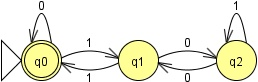
\includegraphics[width=4cm]{./DKAdiv3}

%Regularni izraz po tistem postopku, ki še ni.. reference potem
\ \\
Regularni izraz:
\begin{displaymath}
(0+1(01^*0)^*1)^*
\end{displaymath}
\end{primeri}

\section{Ohranjanje regularnosti jezikov}
Regularnost jezika ohranjajo operacije:
\begin{items}
\item Unija $\cup$
\item Stik $\circ$
\item Iteracija (po Def.)$\ ^*$
\item Presek $\cap$
\item Komplement $\ ^C$ %?rly C
\item Obrat oz. reverz $\ ^R$
\end{items}
Omenimo še nekaj sestavljenih operacij (vse izmed njih ohranjajo regularnost):
\begin{items}
\item Razlika $=\cap^C$%?lol -> \
\item Ekskluzivni ali $\vee=$ %? =?
\end{items}
	
\pagebreak

%?appendix this:
\chapter{Slovar}
%?zihr obstaja neki za to, sicer naredi definitions okolje
\begin{items}
\item Razred - razred je množica elementov, ki ga lahko podamo z naštevanjem elementov ali z opisom lastnosti (opisni ali konceptualni razredi)
\end{items}

\end{document}